\documentclass{article}
\usepackage[utf8]{inputenc}
\usepackage{graphicx}
\usepackage{hyperref}
\usepackage{fancyhdr}
\pagestyle{fancy}

\fancyhead[LE,RO]{Jesse Both}

\hypersetup{
    colorlinks,
    citecolor=black,
    filecolor=black,
    linkcolor=black,
    urlcolor=black
}
\graphicspath{ {/graphics/} }
\title{\Huge{\textbf{CSE 321} \\*  Project 2 \\~\\ \textbf{Count-Down \\* Alarm System}}}
\date{} %remove date from make title


%image

% \begin{center}
% {\includegraphics[height=10cm]{*.png}\centering}
% end{center}

\begin{document}
    \maketitle
    \vfill 
    {\Large\centering\textbf{Jesse Both}\par}
    % {\large\centering{}\par}
    {\large\centering{\today}\par}
    \newpage
    \begin{center}
        \tableofcontents
    \end{center}
\newpage
\setcounter{secnumdepth}{-1}


\section{Introduction}
-
\newline

\section{Specifications}
-
\newline

\section{Featrues}
-
\newline

\section{Applications}
-
\newline

\section{Block Diagram}
-
\newline

\section{Functionality}
-
\newline

\subsection{Bonus Functionality}
-
\newline

\section{Flow Chart}
-
\newline

\section{BOM}
-
\newline

\section{Schematic}
    \begin{center}
        {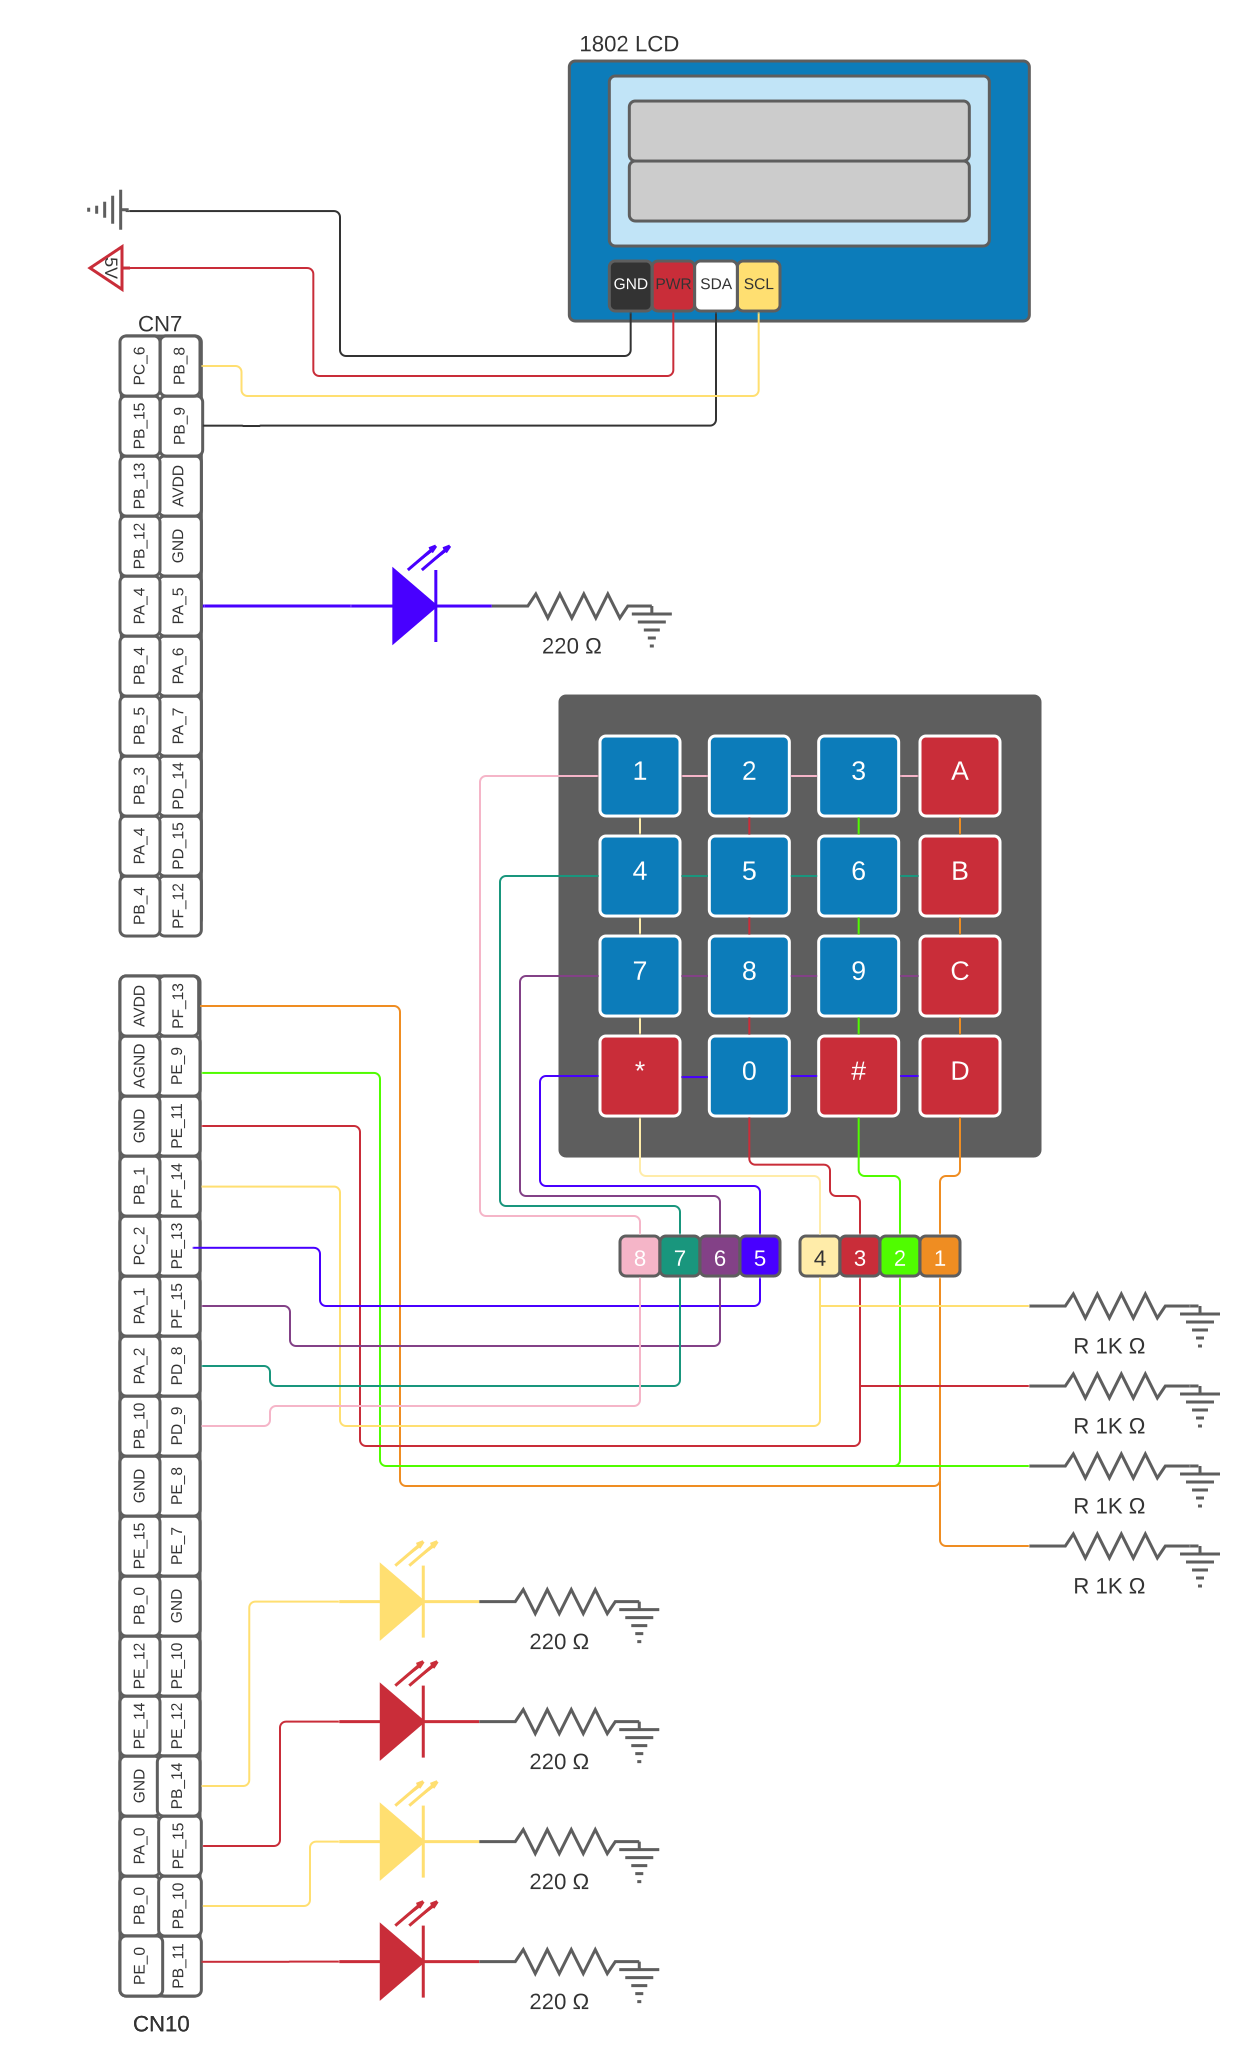
\includegraphics[height=18cm]{graphics/CSE321_project2_schematic.png}\centering} 
    \end{center}
    -
\newline

\section{Test Plan}
-
\newline

\section{Results}
-
\newline

\section{Recommendations}
-
\newline

\end{document}